%%%%%%%%%%%%%%%%%%%%%%%%%%%%%%%%%%%%%%%%%%%%%%%%%%%%%%%%%%%%%%%%%%%%%%
%     File: ExtendedAbstract_imple.tex                               %
%     Tex Master: ExtendedAbstract.tex                               %
%                                                                    %
%     Author: Andre Calado Marta                                     %
%     Last modified : 27 Dez 2011                                    %
%%%%%%%%%%%%%%%%%%%%%%%%%%%%%%%%%%%%%%%%%%%%%%%%%%%%%%%%%%%%%%%%%%%%%%
% A Calculation section represents a practical development
% from a theoretical basis.
%%%%%%%%%%%%%%%%%%%%%%%%%%%%%%%%%%%%%%%%%%%%%%%%%%%%%%%%%%%%%%%%%%%%%%

\section{Analysis}
\label{sec:imple}

%- Granularity benchmark configurations \\
%- Signal and backgrounds \\
%- Boosted category\\
%- Experimental signature\\
%- Optimization \\
%- Event selection \\

The main backgrounds affecting di-Higgs searches in the $b\overline{b}b\overline{b}$ channel are multijet and $t\overline{t}$ production. All other sources of background, including processes involving Higgs bosons, are found to be negligible \cite{hh2bbbbATLAS1}. In addition to these, we also consider the irreducible background ($pp\rightarrow b\overline{b}b\overline{b}$) as a separate background source.

We study the production of Higgs pairs in three different models: the SM, a dark matter (DM) model with a $1$ TeV spin-$0$ mediator that can decay to Higgs pairs \cite{DM} and the CP-conserving Two Higgs Doublet Model (2HDM) of type II where the heavier CP-even Higgs can decay to pairs of SM-like Higgs bosons \cite{2HDM}.

We choose the mass of the new heavy resonances to be high ($\sim 1$ TeV) in order to increase the efficiency of the boosted selection.

\subsection{Simulation setup}
\label{sec:sim}

We simulate the signal and background Monte Carlo samples using a fast simulation workflow. MadGraph5 aMC@NLO \cite{MG5} is used to compute the matrix elements of a given process. Showering and hadronization of colored particles are handled by Pythia8 \cite{Pythia8} and the detector response is parameterized using Delphes3 \cite{Delphes}. 

The irreducible background is generated with an extra jet with $p_T>200$ GeV at generator level ($4b+j$). This guarantees that the pairs of b quarks are boosted enough to increase the probability of being reconstructed as a single, high $p_T$ jet. The multijet background is simulated as $jj+0/1/2~j$ where $j$ stands for a light- or b-initiated jet. To make the simulation more efficient, this background is generated in several $H_T$ regions between $500<H_T<100000$, where $H_T$ is the scalar sum of the $p_T$ of all the partons at generator level. The $t\overline{t}$ background is simulated as $t\overline{t}+0/1/2~j$. The sample is inclusive in the top quark and $W^{\pm}$ boson decay modes.

The BSM signal samples are simulated using MadGraph models publicly available in the FeynRules database. For the DM mediator model \cite{DM}, the spin-$0$ mediator mass is set to $1$ TeV.The cross section for the signal
generated with this model is smaller than the cross section of the SM signal (approximately $0.2$ pb \textit{versus} $0.7$ pb) and therefore this model is not excluded by experimental data.

For the 2HDM \cite{2HDM,2HDM1}, the input parameters for the scalar sector are: 
\begin{align}
&m_{h_1}=125 ~\text{GeV}, \quad m_{h_2}=900 ~\text{GeV},\nonumber \\
&m_{h_3}=850 ~\text{GeV}, \quad m_{hc}=800 ~\text{GeV} \nonumber \\
&mix_{h_2}=mix_{h_3} =0 \nonumber \\
&mix_{h_1}=\frac{\pi}{2}-(\beta-\alpha)\simeq 0.035 \nonumber \\
&l_2\simeq 0.27, \quad l_3\simeq 9.46, \quad l_7\simeq 0.46,
\label{eq:2HDMhiggs_par}
\end{align}
where $m_{h_1}, m_{h_2}, m_{h_3}$ and $m_{h_c}$ are the masses of the three neutral scalars and of the charged scalar, respectively. The mixing angles between the neutral scalars are given by $mix_{h_2}, mix_{h_3}$ and $mix_h$, where we have chosen $\beta=\frac{\pi}{4}$ and $\alpha=-0.75$. $l_{2,3,7}$ are the quartic coupling of the Higgs potential.
All parameters are given in the Higgs basis. Regarding the Yukawa sector, we consider the type II model. The real part of the Yukawa matrices of the coupling of $h_2$ to down $(GDR)$ and up-type $(GUR)$ quarks are given by \cite{2HDM}:
\begin{align}
	&GDR=\text{diag}\left(0,0,\frac{m_b\sqrt{2}\tan(\beta)}{v}\right), \nonumber \\
	&GUR=\text{diag}\left(0,0,\frac{m_b\sqrt{2}}{v\tan(\beta)}\right), \nonumber \\
\end{align}
where $m_b=4.7$ GeV and $m_t=172$ GeV are the masses of the bottom and top quarks. All other matrices are null.  

Different detector configurations were implemented in Delphes3. The granularity of the HCAL was the main study parameter. Starting from the FCC-hh baseline detector, five HCAL granularity benchmark configurations were tested:
\begin{enumerate}
	\item ATLAS HCAL granularity;
	\item Starting from the ATLAS HCAL configuration we increase the granularity in $|\eta|$ by a factor of four, in the pseudorapidity range $\eta < 1.7$ which corresponds to the TileCal region;
	\item Starting from the FCC HCAL configuration we decrease the granularity in $\phi$ by a factor of two, in the entire pseudorapidity range covered by the HCAL;
	\item FCC HCAL default granularity;
	\item Starting from the FCC HCAL configuration we increase the granularity in $\eta$ and in $\phi$ by a factor of two, in the entire pseudorapidity range covered by the HCAL.
\end{enumerate}
These configurations are summarized in table \ref{table:Gran}. In addition, we also passed the same generator level samples through the default ATLAS detector simulation in Delphes. The HCAL granularity is the one that is indicate in the second line of table \ref{table:Gran} but the other detector’s parameters, such as the radius, magnetic field, tracking resolutions are the ones that are implemented in the default ATLAS Delphes card.

\begin{table}
	\centering
	\begin{tabular}{lll}
		\toprule 
		\textbf{Config.} & $\Delta \eta \times \Delta \phi$ & $\eta$ range\\
		\midrule
		\multirow{2}{*}{1} & $0.1\times 0.1$  & $|\eta|<2.5$\\
		& $0.2\times 0.2$ & $2.5<|\eta|<5.0$ \\
		\cellcolor{black!7} &\cellcolor{black!7} $0.025\times 0.1$  & \cellcolor{black!7}$|\eta|<1.7$\\
		\cellcolor{black!7} & \cellcolor{black!7}$0.1\times 0.1$  & \cellcolor{black!7}$1.7<|\eta|<2.5$\\
		\multirow{-3}{*}{2} \cellcolor{black!7}& \cellcolor{black!7}$0.2\times 0.2$  &\cellcolor{black!7} $2.5<|\eta|<5.0$\\
		\multirow{2}{*}{3 }& $0.025\times0.05$ & $|\eta|<2.5$\\
		& $0.05\times 0.1$ & $2.5<|\eta|<6.0$ \\
		\cellcolor{black!7}&  \cellcolor{black!7}$0.025\times0.025$ &  \cellcolor{black!7}$|\eta|<2.5$\\
		\multirow{-2}{*}{4}\cellcolor{black!7}&  \cellcolor{black!7}$0.05\times 0.05$ & \cellcolor{black!7} $2.5<|\eta|<6.0$ \\
		& $0.0125\times0.0125$ &$|\eta|<2.5$\\
		\multirow{-2}{*}{5 }&$0.025\times 0.025$ & $2.5<|\eta|<6.0$\\
		\bottomrule
	\end{tabular}
	\caption{Summary of the benchmark granularity configurations of the HCAL.}
	\label{table:Gran}
\end{table}

\subsection{Event selection}

The event selection targets the boosted kinematic regime in which both Higgs bosons are reconstructed using large-$R$ jets. The expected event topology is illustrated in figure \ref{fig:boosted}.

\begin{figure}[h]
	\centering
	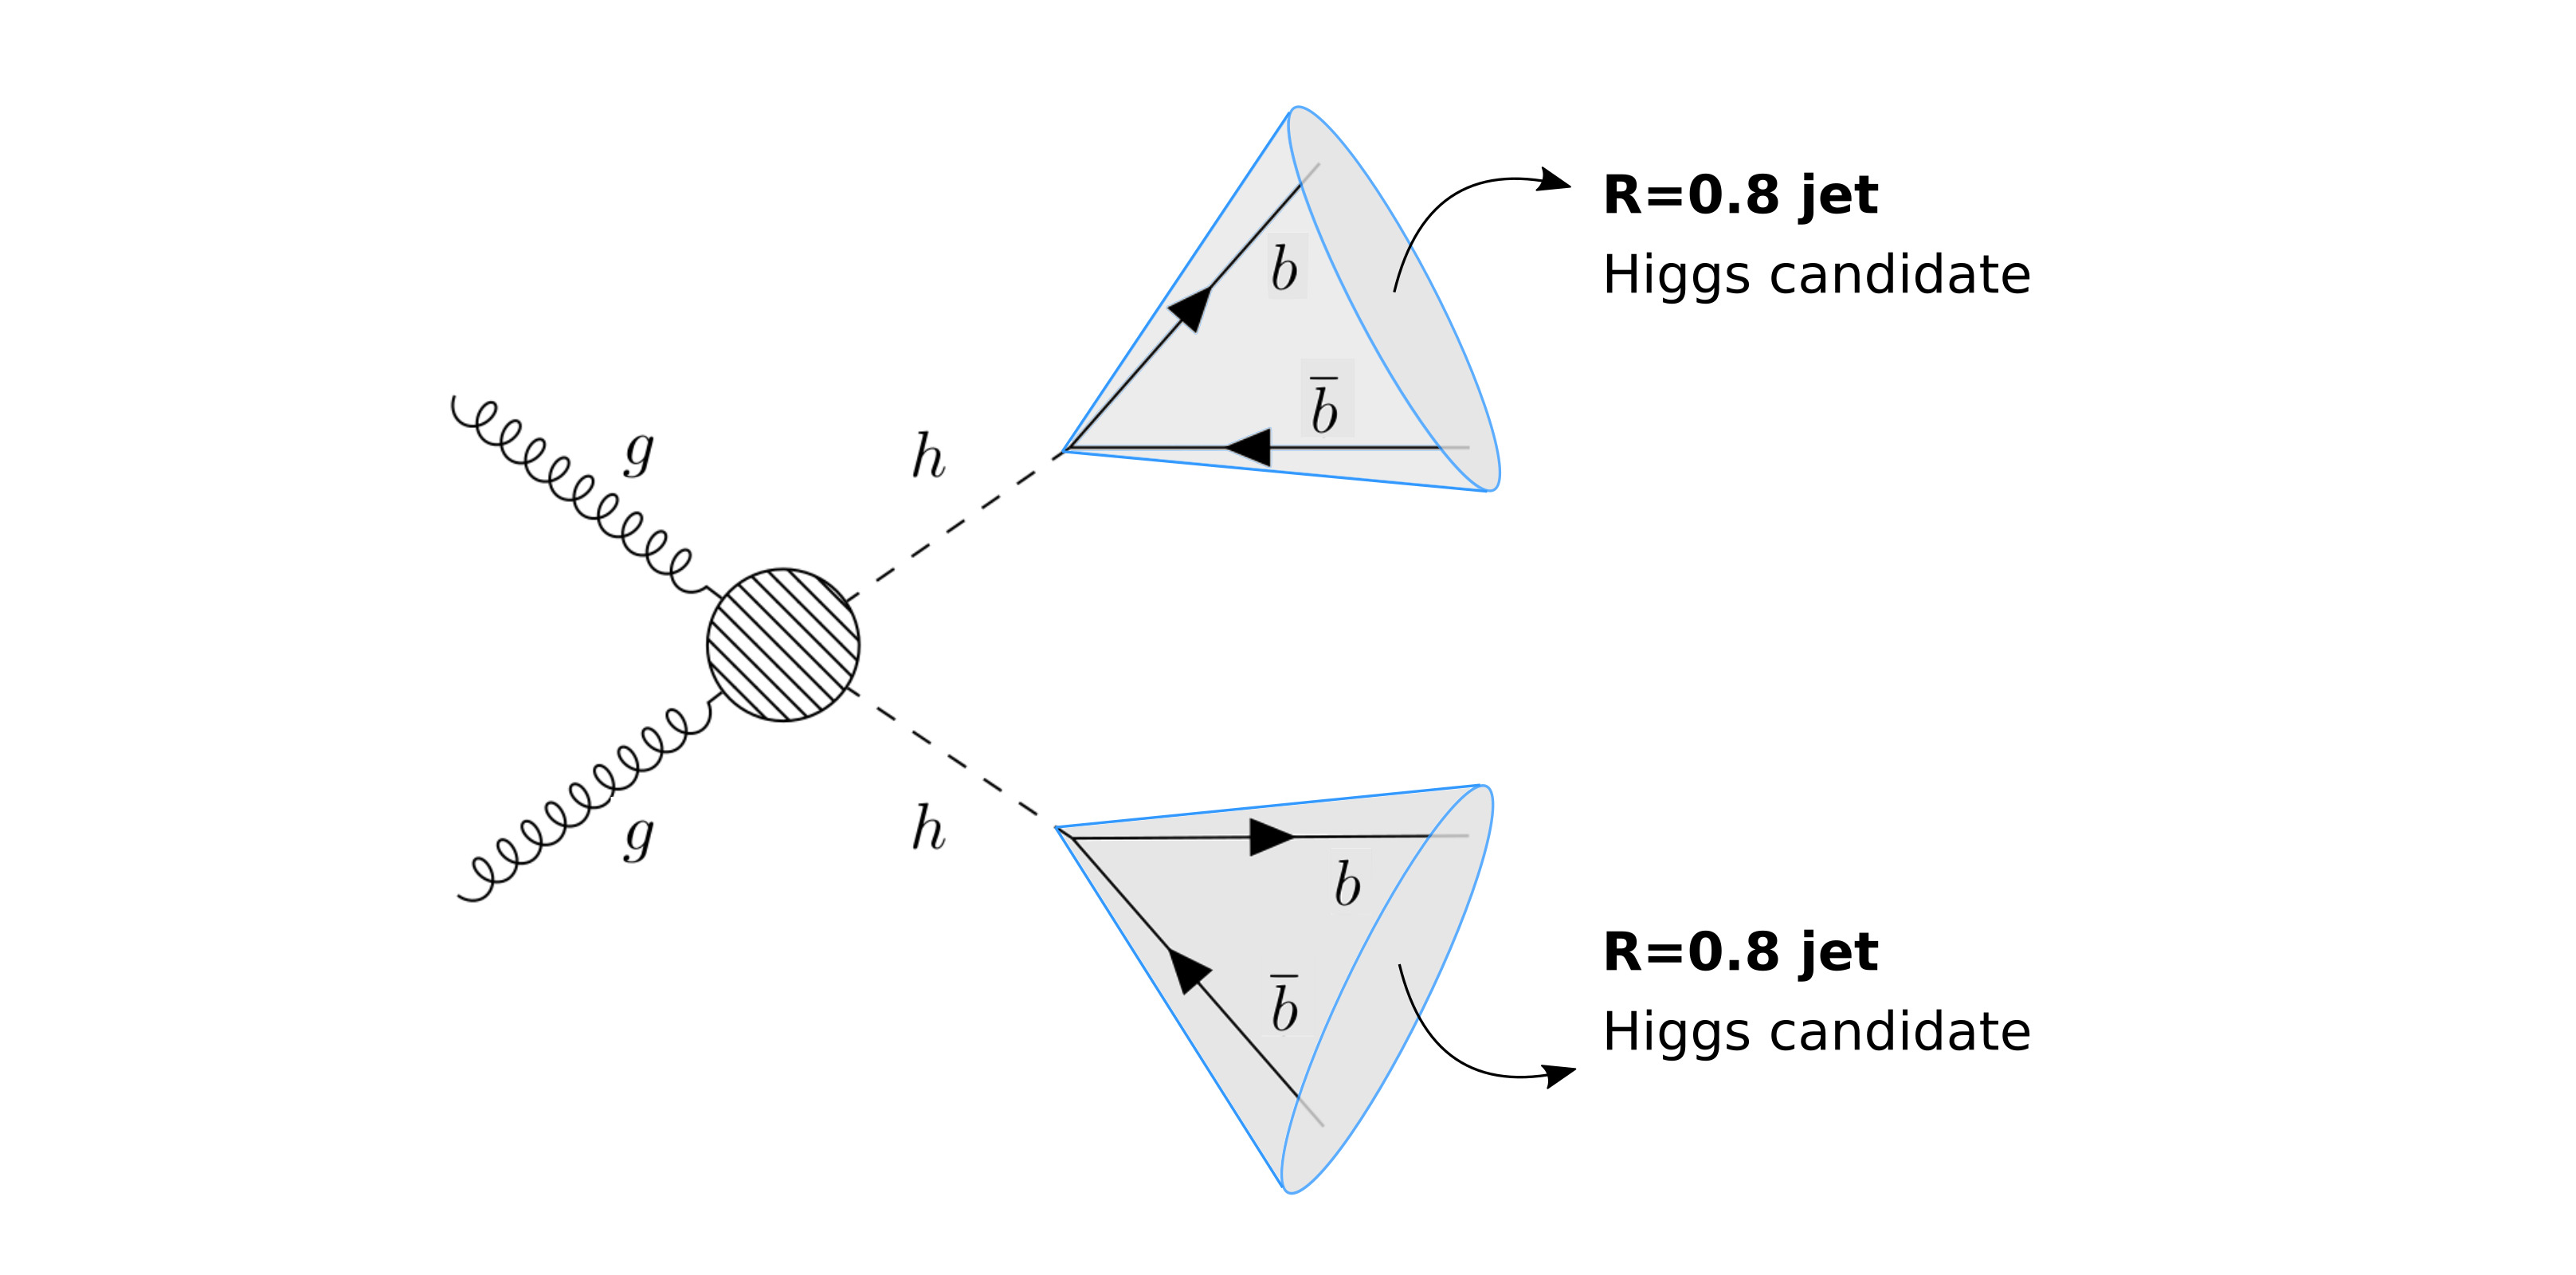
\includegraphics[trim={4.5cm .5cm 1cm .5cm},clip,width=1.2\linewidth]{./images/boosted1.png}
	\caption{Event topology targeted by the boosted analysis region.}
	\label{fig:boosted}
\end{figure}

The events are reconstructed using particle flow (or calorimeter) jets with $R=0.8$ clustered with the anti-$k_T$ algorithm. The events are required to have at least two jets. Each jet is required to have two subjets, both b-tagged. In addition, both jets are required to have $p_T>200$ GeV. These cuts consist of the event pre-selection.

The b-tagging is implemented using truth level information. The b-tagging and mis-tagging efficiencies are extracted from the FCC-hh detector default Delphes card, implemented by the FCC-hh study group. They depend on the $p_T$ and $\eta$ of the jets. The b-tagging efficiency and the c- and light-jet mis-tag rates are of the order of $85\%$, $5\%$ and $1\%$, respectively.

The event selection is described in the following paragraphs. The value of the cuts follow from a simple optimization, done by scanning over a range of possible cut values. This scan is done individually for each of the variables considered. We choose the cut value that maximizes the significance, $S/\sqrt{B}$. 

We require
\begin{equation}
	p_T(h_1)>300~\text{GeV}, \quad p_T(hh)>100 ~\text{GeV}
\end{equation}
where $p_T(h_1)$, $p_T(hh)$ are the transverse momenta of the leading Higgs candidate and of the pair of Higgs candidates, whose distributions can be found in figures \ref{fig:pt_stack}(a) and \ref{fig:pt_stack}(b), respectively.
These cuts help suppress multijet background whose $p_T$ distributions fall more steeply than that of the signal. A requirement on the maximum value of the N-subjetiness variable \cite{Nsubjetiness} of the leading and subleading Higgs candidates, $\tau_{21}(h_1,h_2)$, is imposed to further reject jets that are not consistent with a two-prong substructure:
\begin{equation}
	\tau_{21}(h_1,h_2)<0.4.
\end{equation}
These cuts work as a set of Higgs-tagging criteria, suppressing fake Higgs jets. The distribution of this variable for the leading Higgs is shown in figure \ref{fig:sub_stack}(a). For the signal, the distribution is shifted to lower values.
Since high-mass resonances tend to produce more central jets than multijet background processes, we require:
\begin{equation}
	|\eta(hh)|<1.5,
\end{equation}
where $\Delta\eta(hh)$ is the difference between the pseudorapidities of the two Higgs candidates. This distribution is shown in figure \ref{fig:sub_stack}(b).
We place an additional requirement on the second Fox Wolfram momentum \cite{FW2} of the leading Higgs candidate, $H_2(h_1)$, to further suppress $t\overline{t}$ contamination
\begin{equation}
	H_2(h_1)<0.2.
\end{equation}
This distribution is shown in figure \ref{fig:M_stack}(a) where the large $t\overline{t}$ contribution is visible at values close to zero. 
Events are selected if the softdrop masses, $M_{SD}$, of the large-$R$ jets are consistent with the SM Higgs boson mass
\begin{equation}
	(100<M_{SD}(h_1,h_2)<135) ~\text{GeV}
\end{equation}
This distribution is shown in figure \ref{fig:M_stack}(b), for the leading Higgs candidate. 

\subsection{Systematic uncertainties}

The sources of systematic uncertainty considered are those affecting the signal b-tagging efficiency and the normalization of the backgrounds. These are the dominant uncertainties in the search for boosted $hh\rightarrow b\overline{b}b\overline{b}$ \cite{hh2bbbbATLAS1} and rough estimates of their size are extracted from the literature. In the four b-tags signal region, the uncertainty on the b-tagging is of the order of $30\%$ \cite{hh2bbbbATLAS1}. For the normalization of the QCD multijet and $t\overline{t}$ backgrounds we consider uncertainties of $50\%$ and $20\%$, respectively \cite{FCCphysClement}.

The b-tagging uncertainty is implemented by varying the number of signal events up and down by $30\%$. The normalization of the QCD multijet ($4b+j$ and $jj+0/1/2~j$) and $t\overline{t}$ is varied independently by the corresponding factors. The systematic uncertainties are considered to be uncorrelated and therefore the variations to the nominal value of $S/\sqrt{B}$ are added in quadrature.

\begin{figure*}
	\centering
	\begin{minipage}{.5\textwidth}
		\centering
		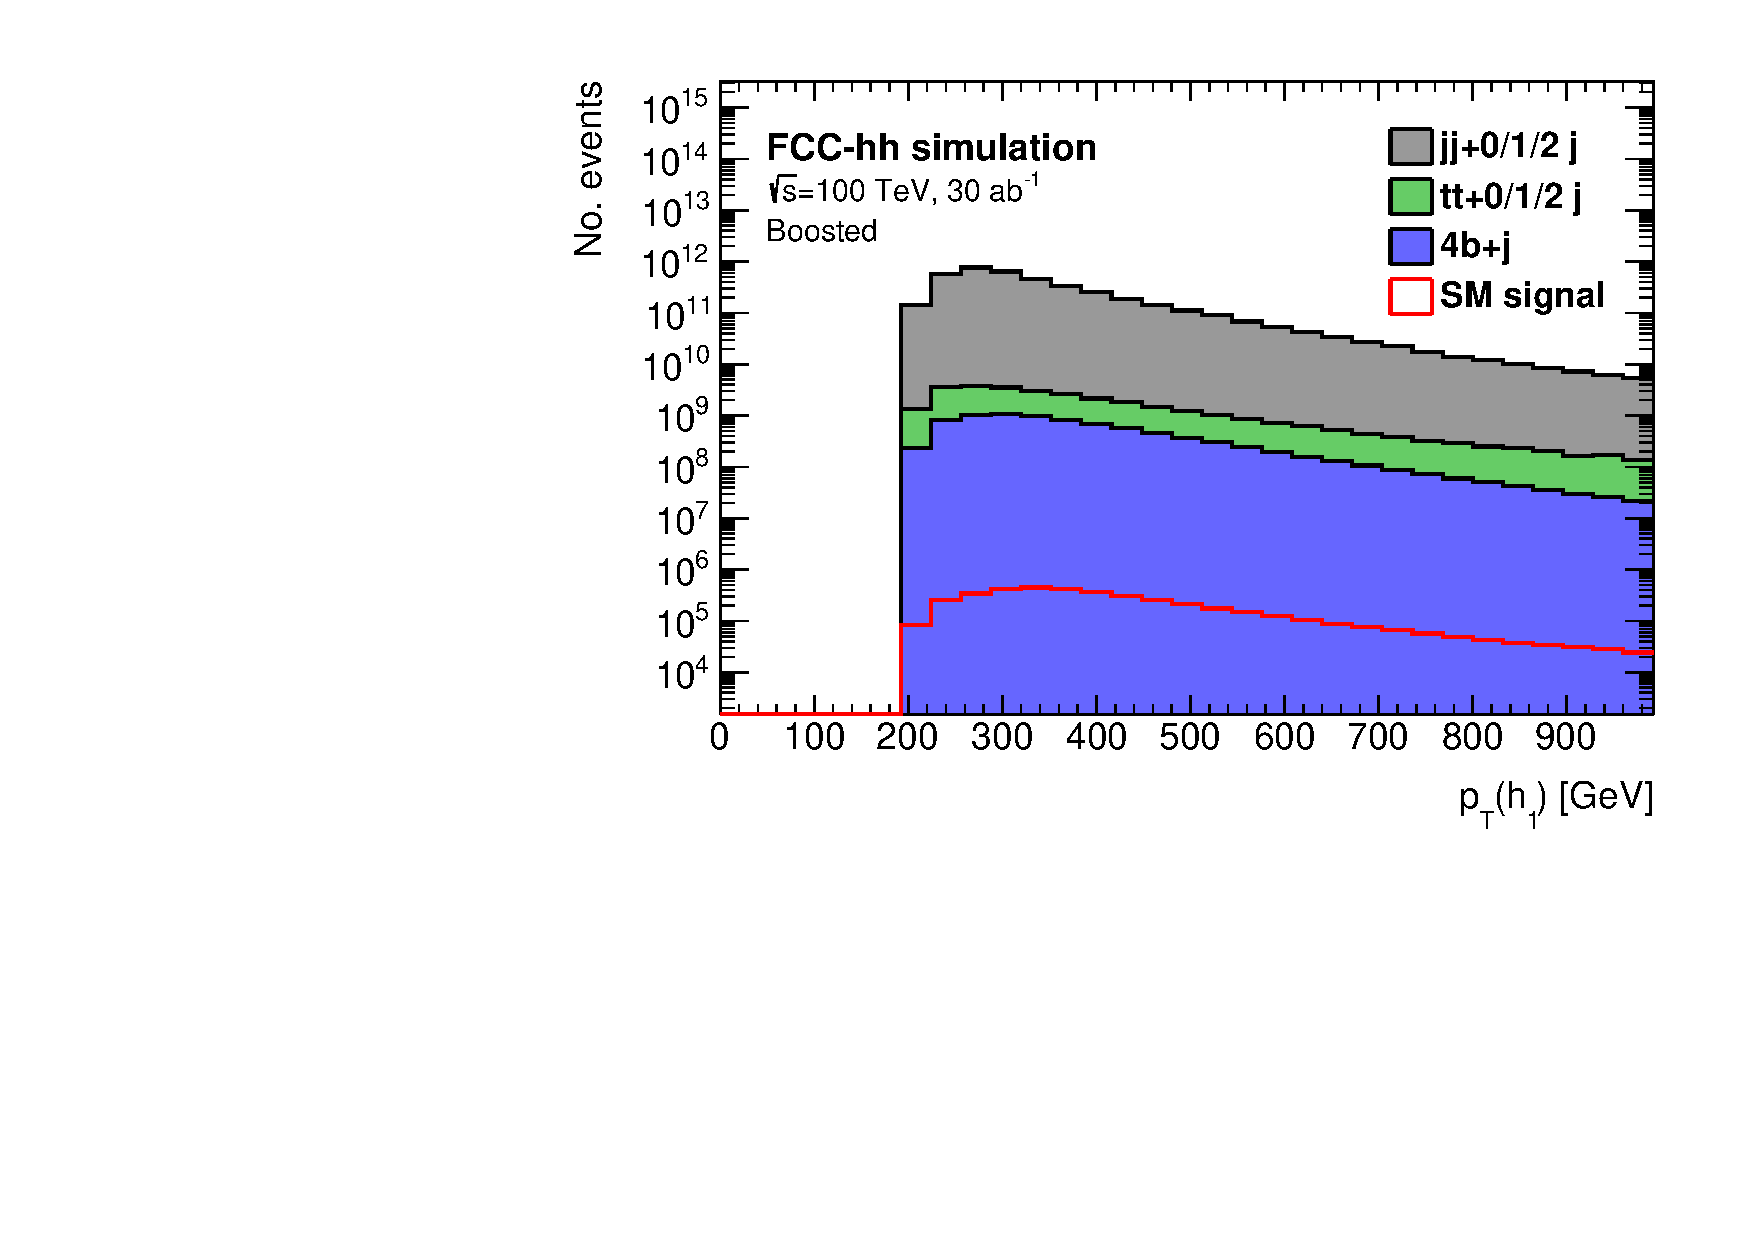
\includegraphics[width=\linewidth]{./images/hist_h1_pt_stack.pdf}
	\end{minipage}%
	\begin{minipage}{.5\textwidth}
		\centering
		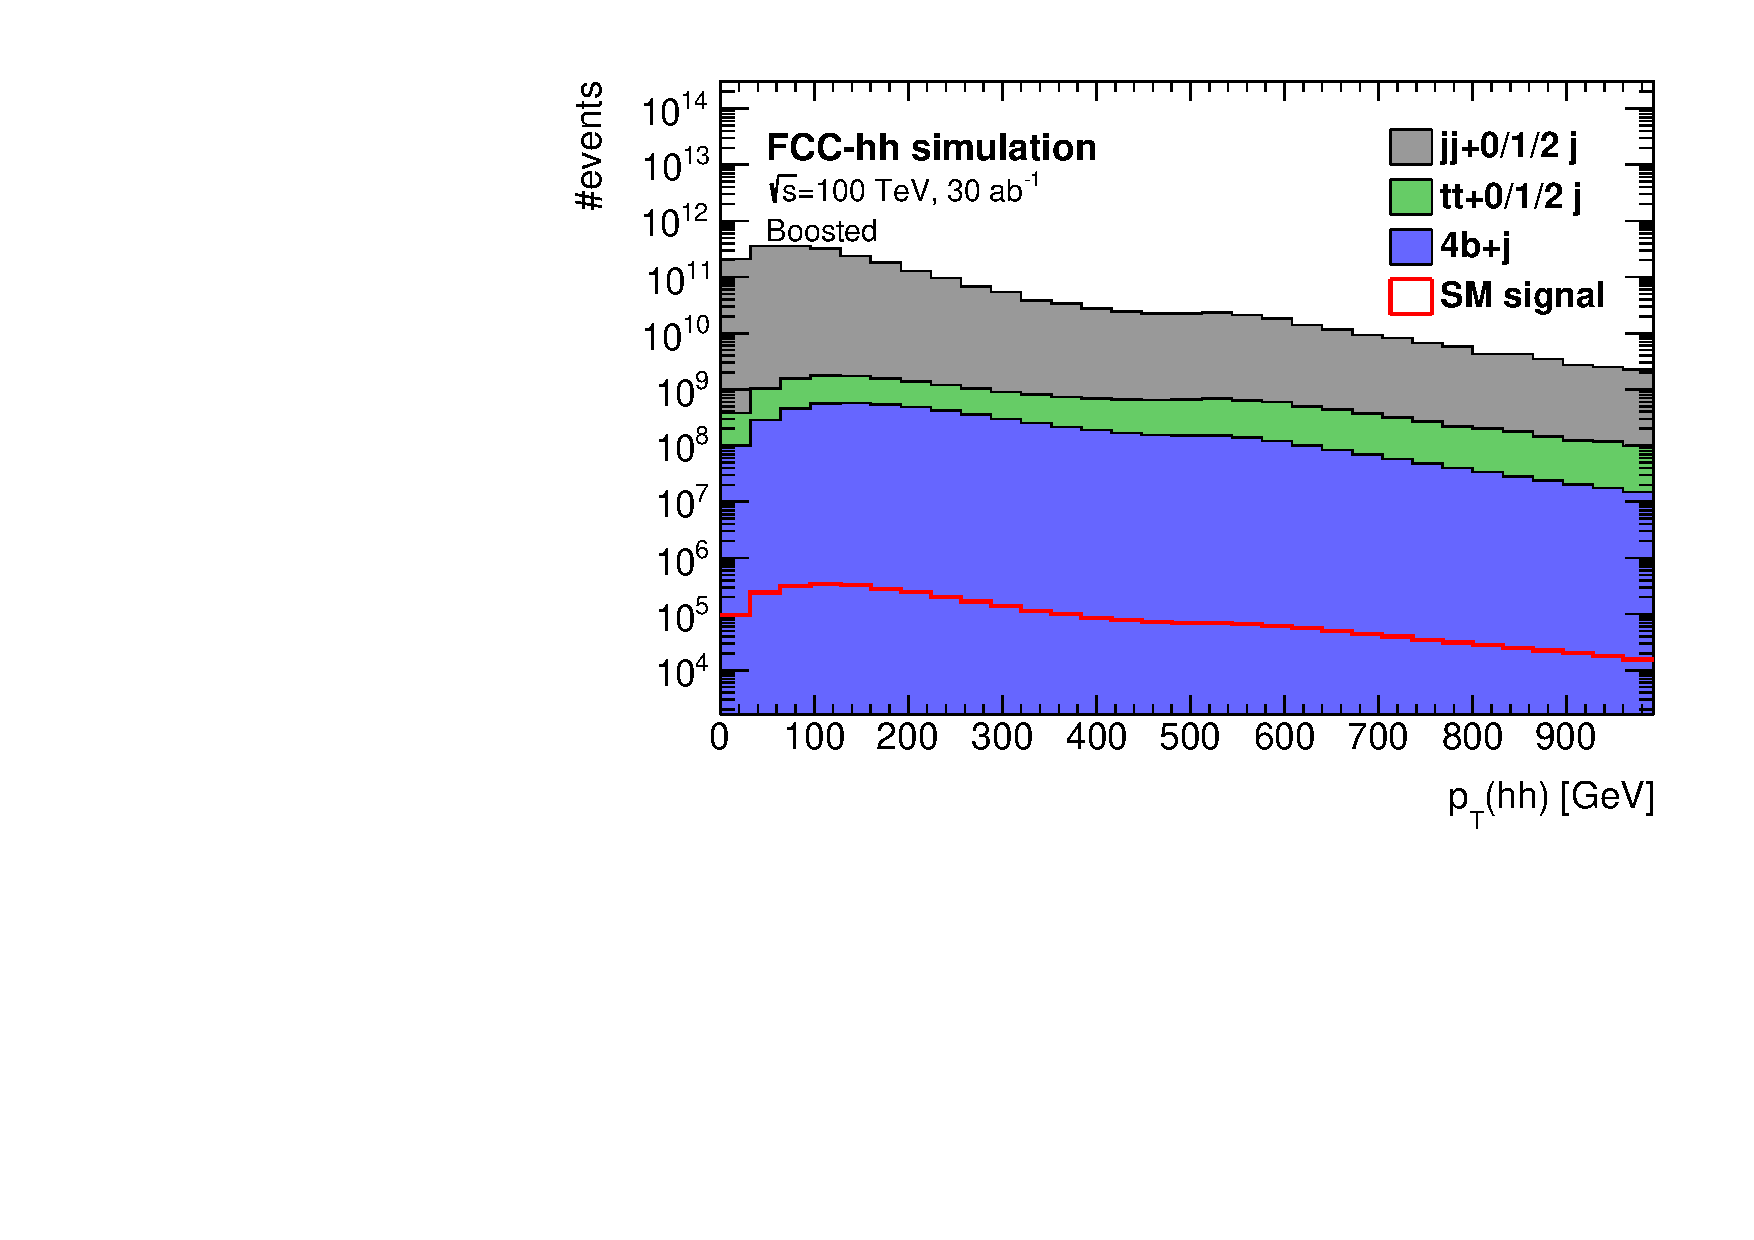
\includegraphics[width=\linewidth]{./images/hist_hh_pt_stack.pdf}
	\end{minipage}
	\begin{minipage}[t]{0.5\textwidth}
		\caption*{(a)}
		%\label{fig1}
	\end{minipage}%%%
	\hfill
	\begin{minipage}[t]{0.5\textwidth}
		\caption*{(b)}
		%\label{fig2}
	\end{minipage}
	\caption{(a) $p_T$ distributions of the leading Higgs candidate, $p_T(h_1)$, after the pre-selection cuts, (b) $p_T$ distribution of the Higgs pair, $p_T(hh)$, after the cut on $p_T(h_1)>300$ GeV.}
	\label{fig:pt_stack}
\end{figure*}

\begin{figure*}
	\centering
	\begin{minipage}{.5\textwidth}
		\centering
		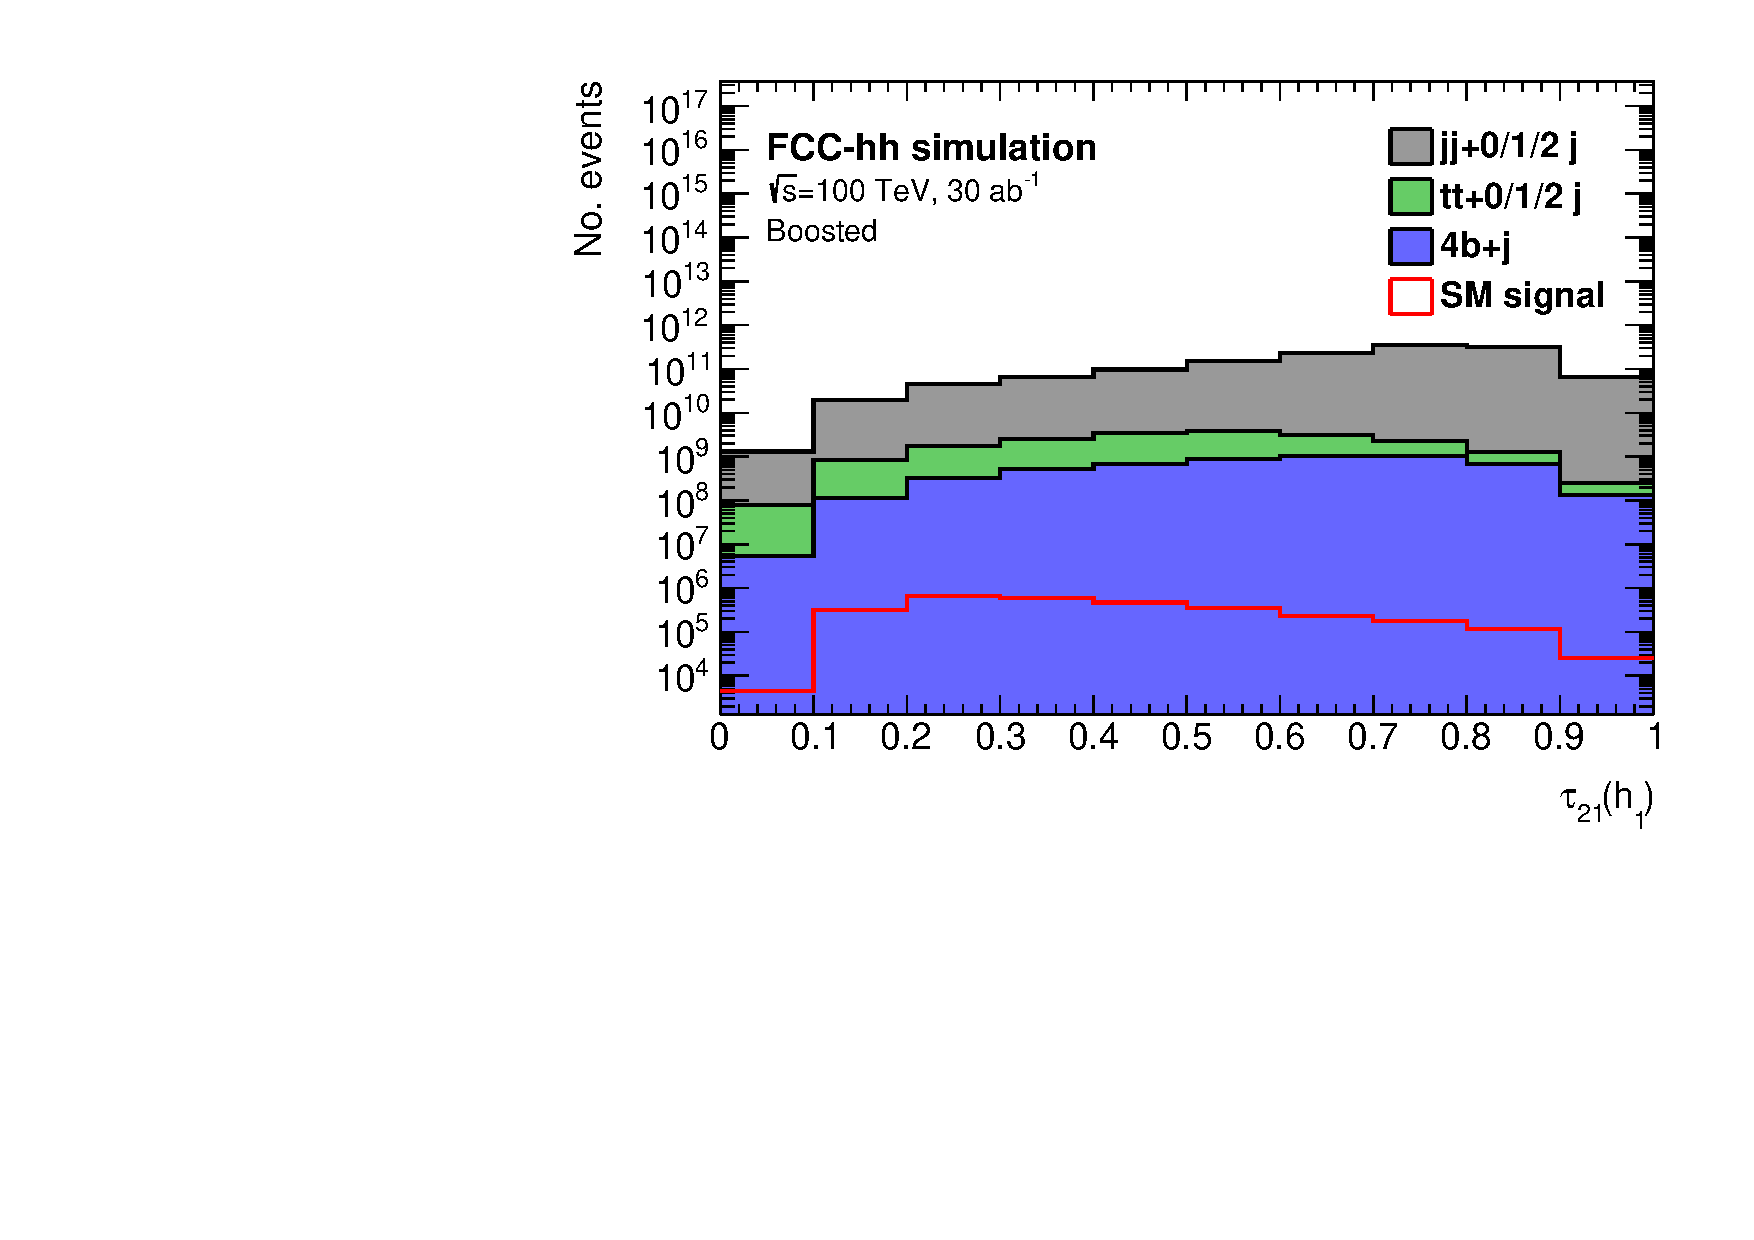
\includegraphics[width=\linewidth]{./images/hist_h1_tau21_stack.pdf}
	\end{minipage}%
	\begin{minipage}{.5\textwidth}
		\centering
		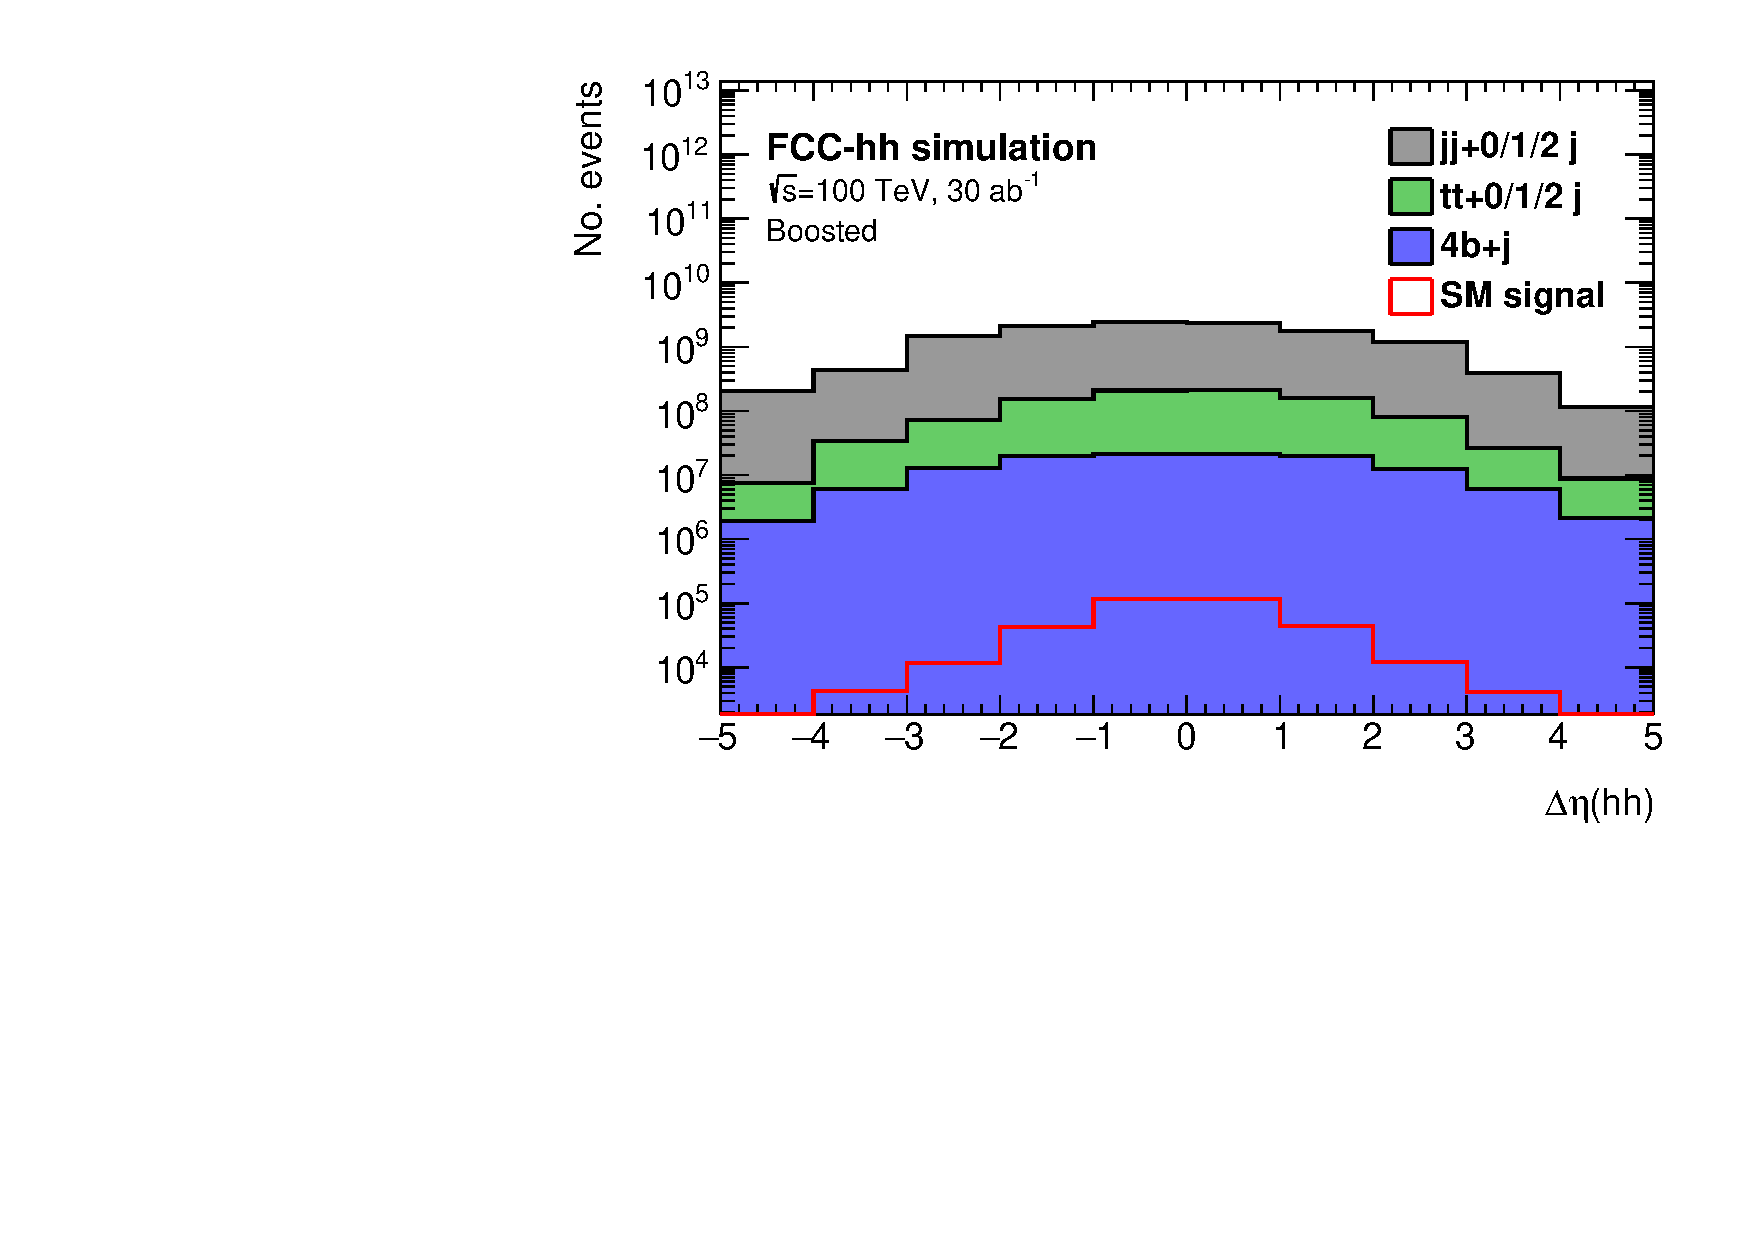
\includegraphics[width=\linewidth]{./images/hist_hh_deltaEta_stack.pdf}
	\end{minipage}
	\begin{minipage}[t]{0.5\textwidth}
		\caption*{(a)}
		%\label{fig1}
	\end{minipage}%%%
	\hfill
	\begin{minipage}[t]{0.5\textwidth}
		\caption*{(b)}
		%\label{fig2}
	\end{minipage}
	\caption{(a) $\tau_{21}$ distribution for the leading Higgs candidate, $\tau_{21}(h_1)$, after the cut on $p_T(hh)>100$ GeV, (b) Distribution of the $\Delta\eta$ between the two Higgs candidates, $\Delta\eta(hh)$, after the cuts on $\tau_{21}(h_1,h_2)<0.4$.}
	\label{fig:sub_stack}
\end{figure*}

\begin{figure*}
	\centering
	\begin{minipage}{.5\textwidth}
		\centering
		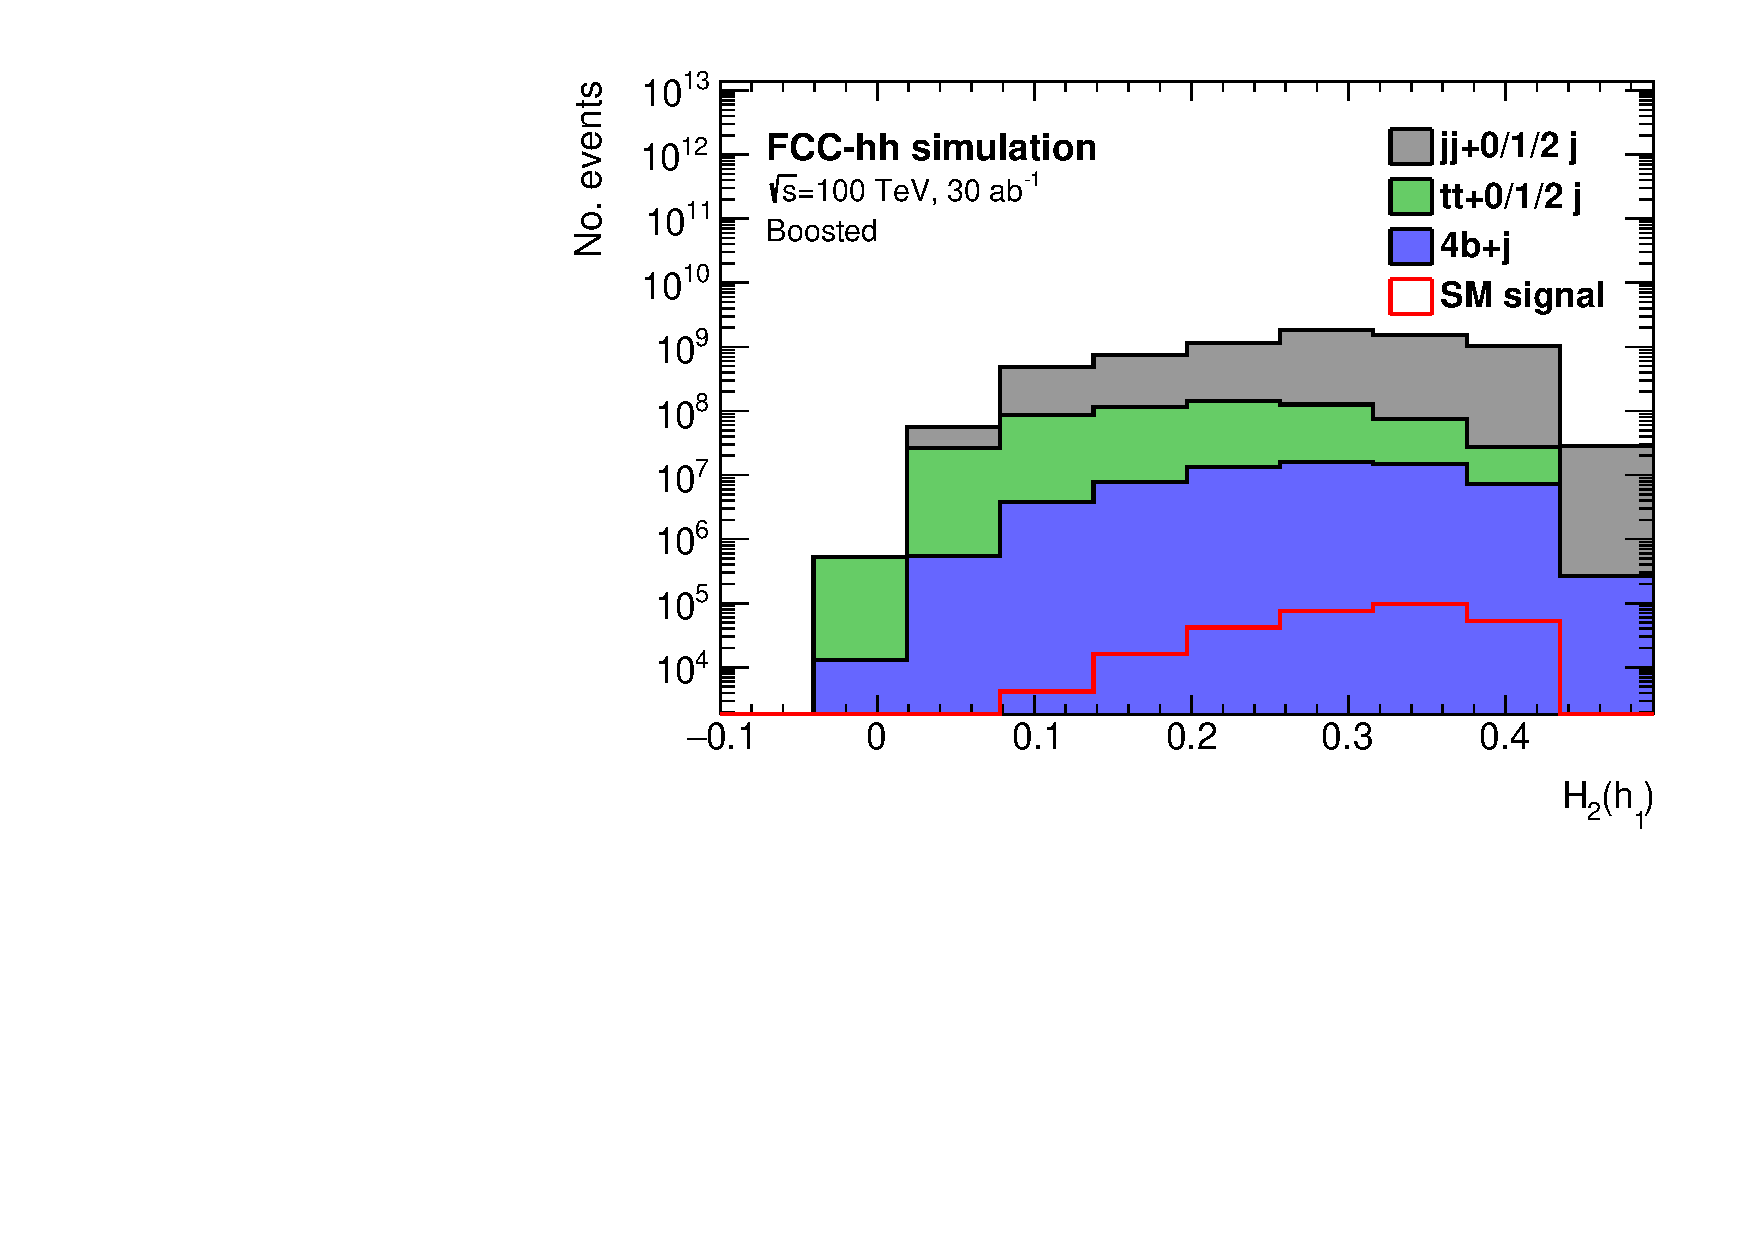
\includegraphics[width=\linewidth]{./images/hist_h1_FW2_stack.pdf}
	\end{minipage}%
	\begin{minipage}{.5\textwidth}
		\centering
		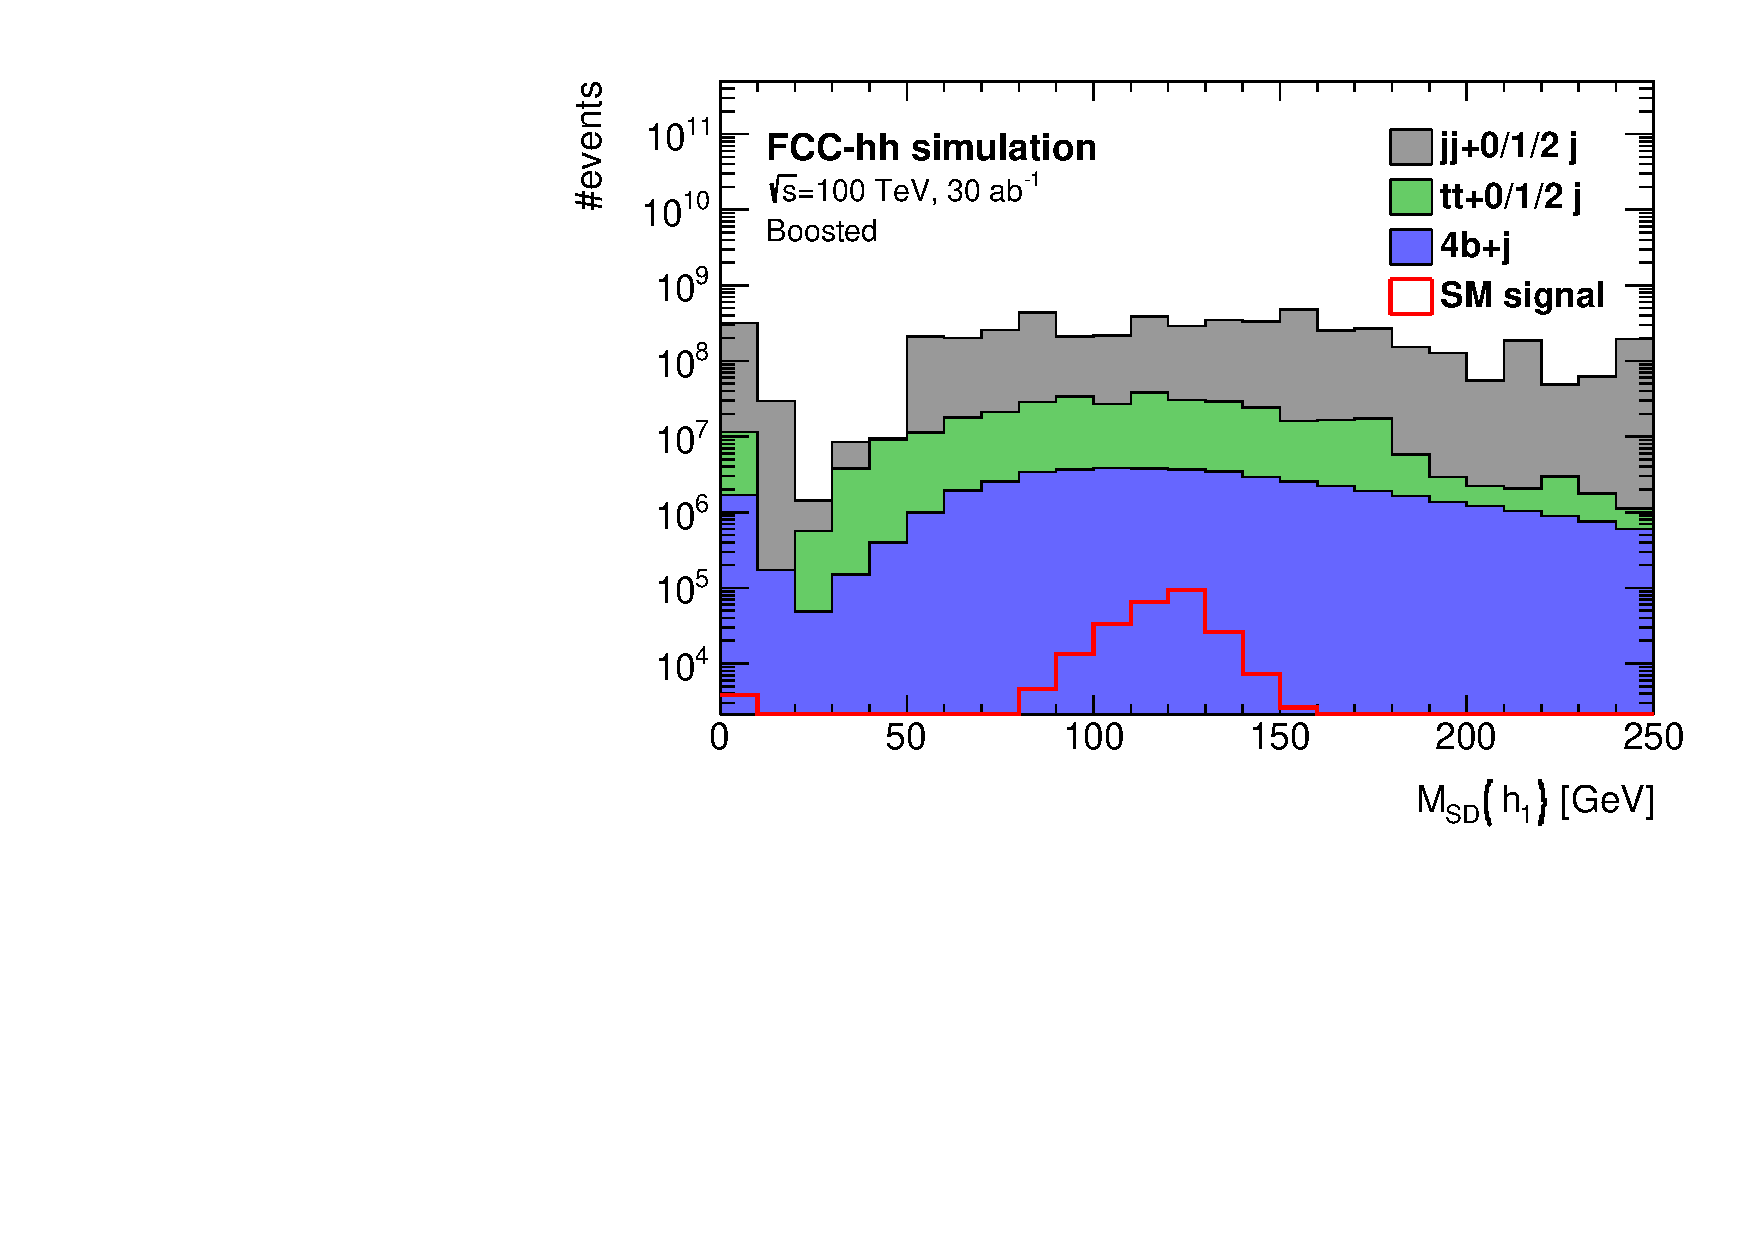
\includegraphics[width=\linewidth]{./images/hist_h1_softdrop_M_stack.pdf}
	\end{minipage}
	\begin{minipage}[t]{0.5\textwidth}
		\caption*{(a)}
		%\label{fig1}
	\end{minipage}%%%
	\hfill
	\begin{minipage}[t]{0.5\textwidth}
		\caption*{(b)}
		%\label{fig2}
	\end{minipage}
	\caption{(a) Distribution of the second Fox-Wolfram momentum of the leading Higgs candidate, $H_2(h_1)$, after the cut $|\Delta\eta(hh)|<1.5$, (b) Softdrop mass distribution for the leading Higgs candidate, $M_{SD}(h_1)$, after the cut $H_2(h_1)>0.2$.}
	\label{fig:M_stack}
\end{figure*}

%
%\begin{figure}[h]
%	\centering
%	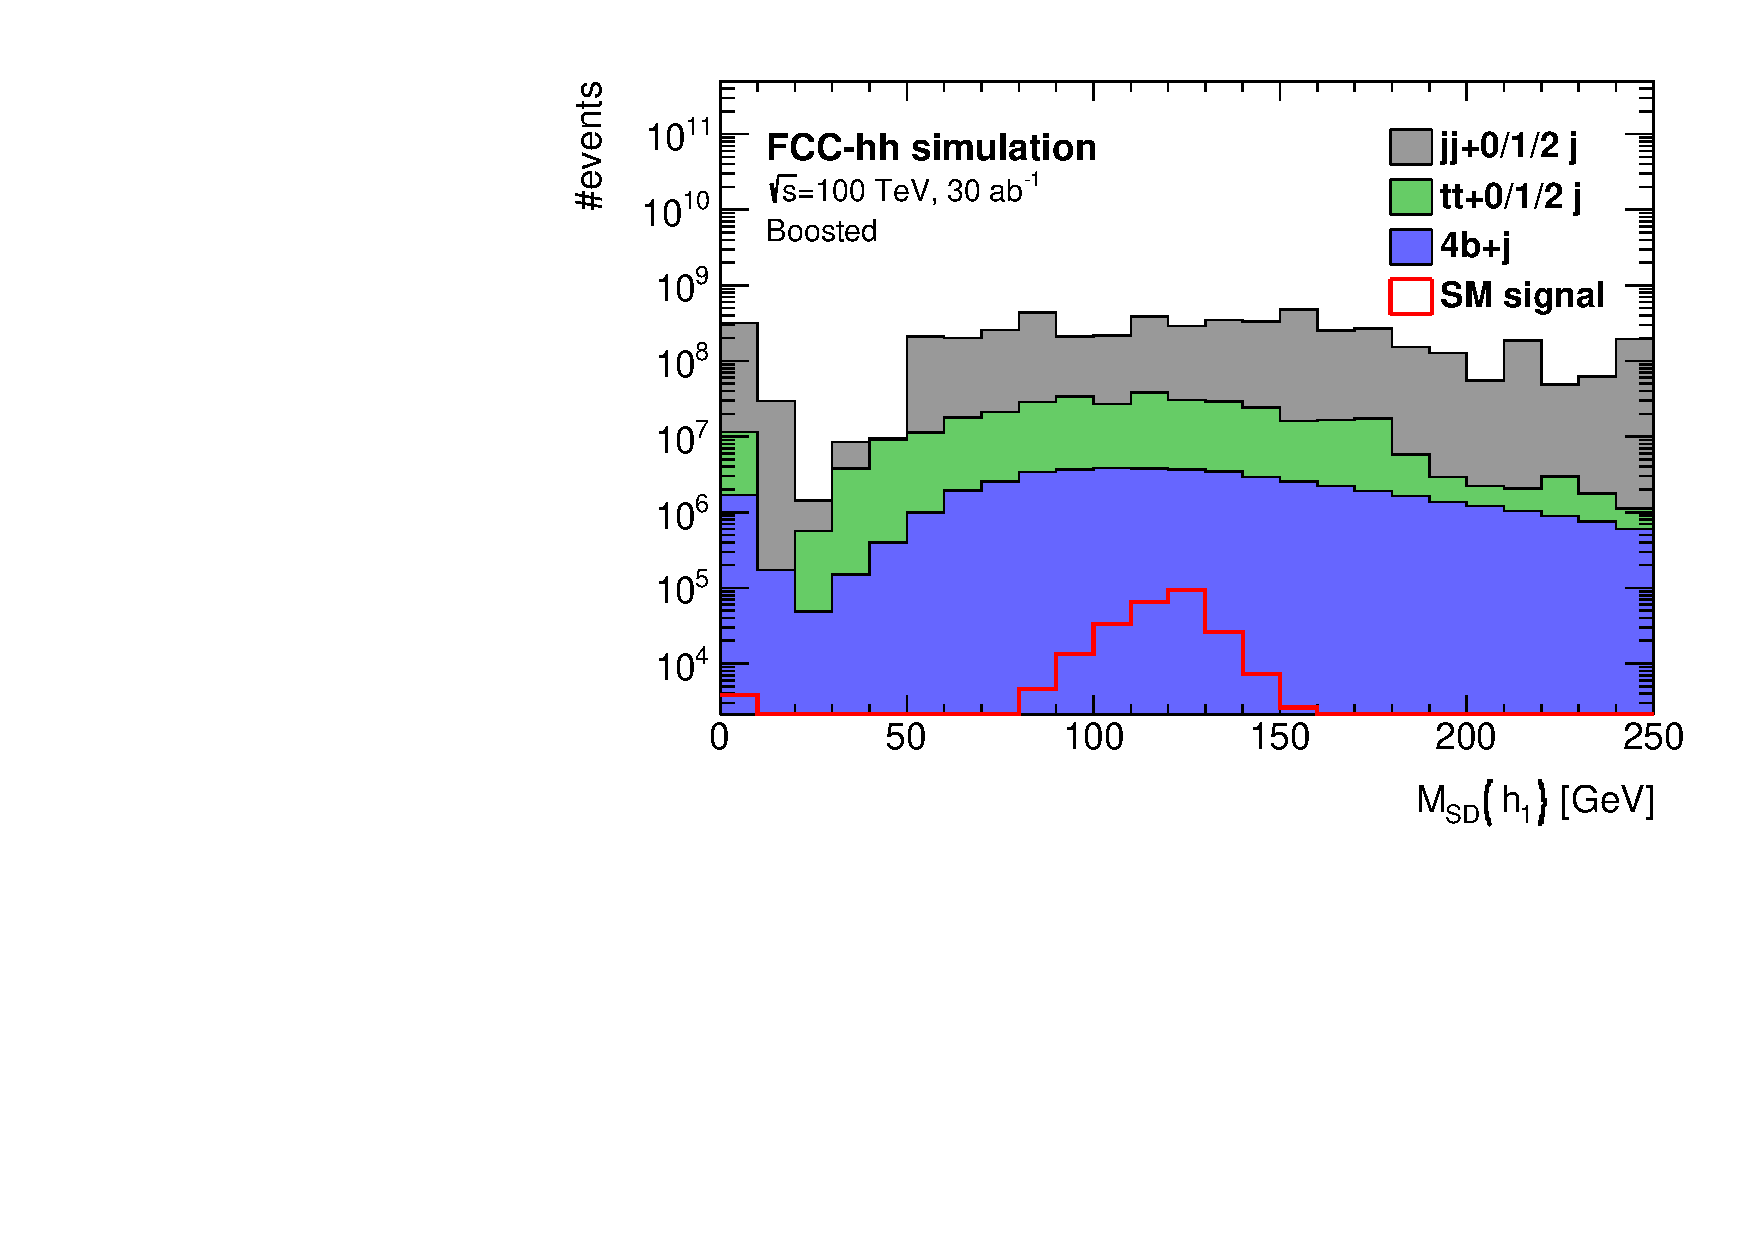
\includegraphics[width=\linewidth]{./images/hist_h1_softdrop_M_stack.pdf}
%	\label{fig:stack}
%	\caption{oi}
%\end{figure}


